%% ASP.NET MVC Architecture

\section{ASP.NET MVC architektúra}

\indent Az államvizsga-dolgozatom célja bemutatni egy webalapú alkalmazás fejlesztési folyamatát és technológiai hátterét, amely egy buszvállalat működését támogatja. A fejlesztés során az ASP.NET MVC keretrendszerre építek, amely jól strukturált megközelítést kínál a webes alkalmazások építéséhez, miközben lehetővé teszi az üzleti logika, a megjelenítés és az adatkezelés hatékony szétválasztását.

A dolgozat első fejezete a .NET platform által kínált lehetőségekre és az MVC (Model-View-Controller) architektúra alapelveire összpontosít. Részletesen ismertetjük a modell, a nézet és a vezérlő szerepét, valamint ezek együttműködését a rendszer működésében. Külön figyelmet fordítunk az útvonalkezelés és az adatátadás mechanizmusaira is, amelyek az ASP.NET MVC egyik kulcsfontosságú komponensét jelentik.

A következő alfejezetekben bemutatásra kerülnek azok a technológiák, amelyek kiegészítik és támogatják az alkalmazás működését. Az Entity Framework révén az adatbázis-kezelés objektumorientált módon valósul meg, míg a Razor nézetmotor a dinamikus tartalmak hatékony megjelenítését teszi lehetővé. A kliensoldali működéshez elengedhetetlen JavaScript mellett a Leaflet könyvtár térképes vizualizációt biztosít, amely különösen hasznos a szállítási útvonalak megjelenítéséhez. A rendszer részeként implementált e-mail értesítések SMTP protokollon keresztül működnek, míg a QR-kód generálás lehetőséget nyújt például jegyek, csomagazonosítók vagy beléptetési információk digitális tárolására és gyors elérésére.

\begin{figure}[H]
    \centering
    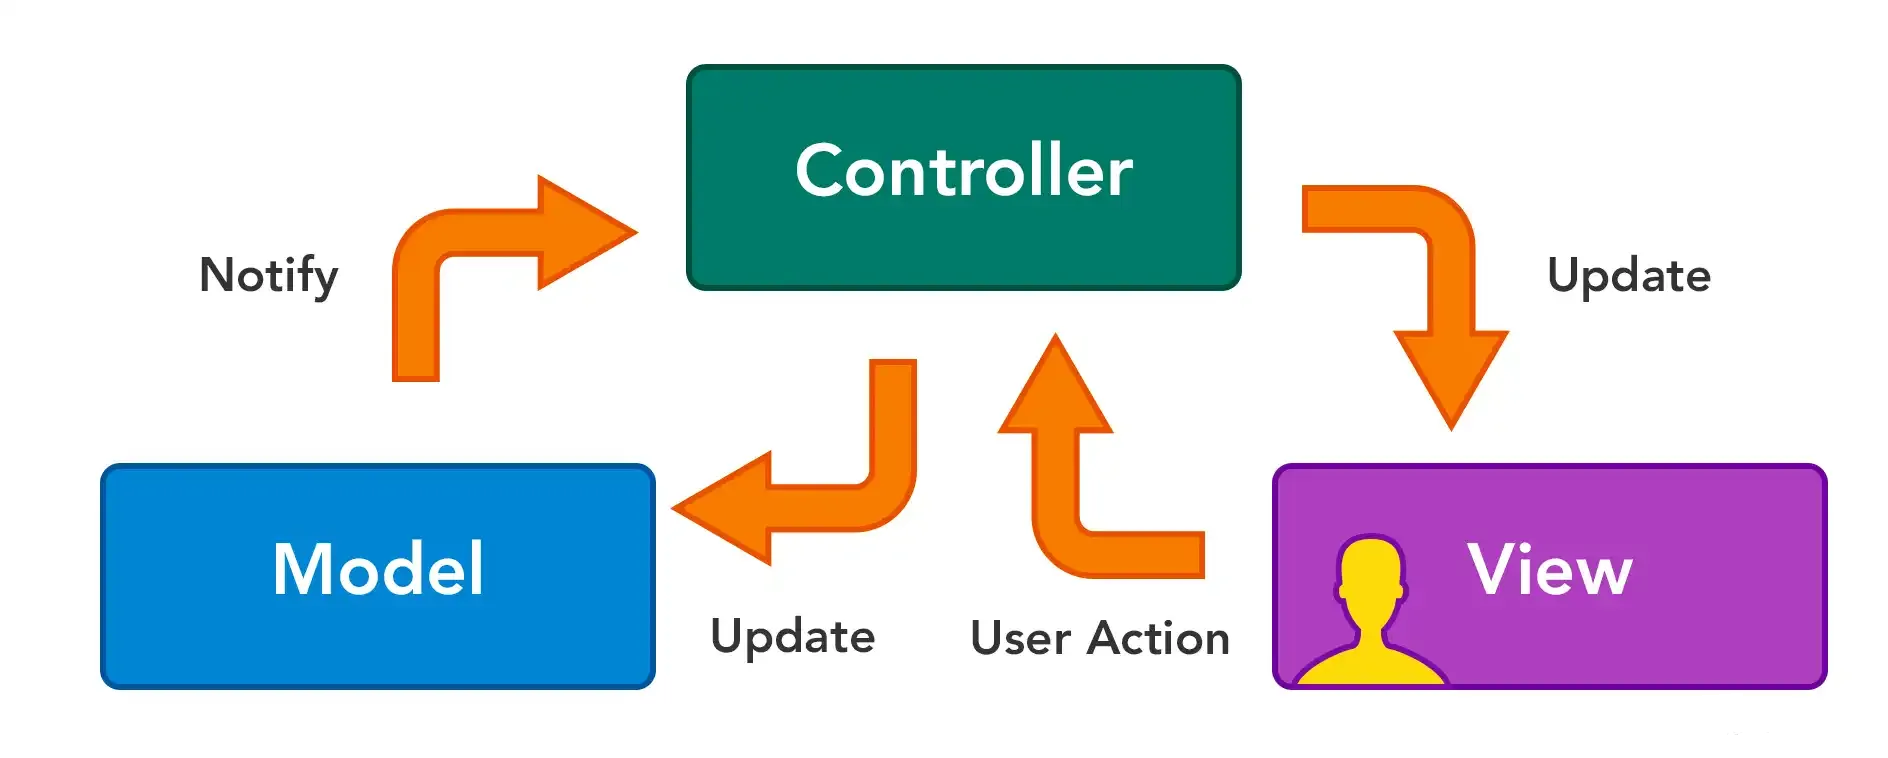
\includegraphics[width=1\textwidth]{Szakdolgozat/Mellekletek/MVCDiagramm.png}
    \caption{Az MVC (Model–View–Controller) architektúra felépítése. Az ábrán jól látható, hogyan különül el az adatkezelés (Model), a felhasználói felület (View) és az üzleti logikát kezelő vezérlő (Controller). Az egyes rétegek közötti kommunikáció segíti az alkalmazás moduláris, karbantartható és tesztelhető kialakítását.}
    \label{fig:er-diagram}
\end{figure}


\subsection{A .NET platform és az MVC minta}

\indent A .NET egy többnyelvű, keresztplatformos fejlesztési környezet, amelyet a Microsoft hozott létre, és amely lehetőséget nyújt különböző típusú alkalmazások – például asztali, webes és mobil – fejlesztésére. A platform célja, hogy egységes, megbízható és jól skálázható környezetet biztosítson a fejlesztők számára. Ezen belül az ASP.NET a webalkalmazások készítésére szolgáló keretrendszer, amely támogatja az MVC (Model–View–Controller) mintát.

Az MVC architektúra egyik legfontosabb előnye az alkalmazás logikájának, adatainak és felhasználói felületének elkülönítése. Ez nemcsak a kód tisztaságát és átláthatóságát javítja, hanem lehetővé teszi a különböző fejlesztői szerepkörök (pl. backend, frontend) hatékony együttműködését, valamint a rendszer egyszerűbb tesztelhetőségét és karbantarthatóságát.

\subsubsection{ASP.NET MVC alapelvei}

\indent Az ASP.NET MVC keretrendszer három jól elkülöníthető rétegre bontja az alkalmazás struktúráját. A Model réteg felelős az üzleti logika és az adatok kezeléséért, a View a felhasználó számára megjelenített tartalmat írja le, míg a Controller a két réteg közötti kommunikációért és az események kezeléséért felel. Ez az elkülönítés elősegíti az egységek külön történő fejlesztését és tesztelését.

Az ASP.NET MVC a REST architektúra alapelveit követi, és szorosan épít az URL-alapú útvonalkezelésre (routing), amely meghatározza, hogy egy adott kérés melyik vezérlőhöz és metódushoz kerüljön.

\subsubsection{A Controller, View és Model szerepe}

\indent A Controller felelős a beérkező HTTP-kérések kezeléséért, az adatok lekérdezéséért vagy módosításáért, és végül az adatok továbbításáért a View felé. A Model tartalmazza az alkalmazás által kezelt adatokat és azok viselkedését, gyakran adatbázissal kapcsolatban álló entitások és azok logikája formájában. A View Razor szintaxisban írt .cshtml fájlokat jelent, amelyek HTML-ben jelenítik meg a Modelből származó adatokat, ezzel biztosítva a dinamikus tartalom megjelenítését.

\subsubsection{Routing és adatátadás}

\indent Az útvonalkezelés (routing) kulcsszerepet játszik az ASP.NET MVC működésében. Az URL-ek mintákat követnek, amelyek alapján a rendszer eldönti, hogy melyik Controller és azon belül melyik Action metódus hajtódjon végre. Az adatok átadása történhet route paramétereken, query stringen vagy formokon keresztül, míg az adatok feldolgozását és továbbítását a Controller végzi, amely továbbküldi azokat a View vagy más üzleti logikai rétegek számára.

\subsection{Kapcsolódó technológiák}

\subsubsection{Entity Framework és az adatkezelés integrációja}

\indent Az Entity Framework (EF) a .NET keretrendszer objektum-relációs leképezést (ORM) alkalmazó technológiája, amely lehetővé teszi, hogy az adatbázis-műveleteket magas szintű, típusosan definiált C\# osztályokon keresztül végezzük el. Az EF célja, hogy a relációs adatbázisokkal való munka során elrejtse a nyers SQL lekérdezések szükségességét, ezáltal elősegítve a biztonságosabb és karbantarthatóbb adatkezelést.

Az EF támogatja a különböző adatmodellezési megközelítéseket, köztük a Code First és Database First stratégiákat. A Code First megközelítés lehetővé teszi, hogy a fejlesztők először az osztálystruktúrát hozzák létre a C\# nyelv eszközeivel, majd az EF automatikusan létrehozza és karbantartja a hozzá tartozó adatbázis-sémát. Ezzel szemben a Database First modell olyan helyzetekben előnyös, ahol már létező adatbázis-struktúrához kell alkalmazkodni.

Az alkalmazás adatbázis-kommunikációja általában Microsoft SQL Serverrel történik, amely a .NET ökoszisztémán belül natívan támogatott. Az EF SQL Serverrel való összekapcsolását a DbContext konfigurálásán keresztül végezzük, ahol a kapcsolat elérési adatai (connection string) egy konfigurációs fájlban vagy programkódban definiálhatók. A kapcsolat biztonságos kezeléséhez jellemzően Windows hitelesítést vagy SQL Server hitelesítést használunk, opcionálisan SSL titkosítással.

A modern ASP.NET alapú alkalmazásokban az EF szorosan együttműködik az ASP.NET Identity keretrendszerrel, amely a felhasználókezelési és hitelesítési feladatokat látja el. Az Identity rendszer szintén az EF-en keresztül valósítja meg a felhasználói adatok (pl. regisztrációs információk, jelszavak hash-elve, jogosultságok, szerepkörök) tartós tárolását és kezelését. A felhasználói entitások a többi modellosztályhoz hasonlóan entitásként jelennek meg az adatbázisban, így az EF által biztosított LINQ-lekérdezések és migrációs eszközök teljes mértékben alkalmazhatók rájuk is.

Ez az integrált megközelítés lehetővé teszi, hogy az alkalmazás egységes módon kezelje mind az üzleti, mind az autentikációs adatokat, miközben biztosítja az adatbázis-struktúra automatikus frissítését és bővítését a fejlesztés során.

\subsubsection{Razor nézetek}

\indent A Razor egy modern, egyszerű szintaxisú nézetmotor, amely a HTML és C\# nyelv elemeit ötvözi. Lehetővé teszi, hogy a dinamikus tartalom hatékonyan jelenjen meg a felhasználói felületen, miközben a kód jól olvasható marad. A Razor nézetek általában {.cshtml} kiterjesztésű fájlokban jelennek meg, és az alkalmazás prezentációs rétegének meghatározó elemei.

\indent A megjelenítés esztétikai és felhasználói élménybeli szempontból történő javítása érdekében a Razor nézetekben gyakran alkalmazzák a Bootstrap keretrendszert, amely előre definiált, reszponzív stílusokat és elrendezéseket kínál. Emellett elterjedt a Bootstrap Icons (BI) használata is, amely vektor alapú ikonokat biztosít a vizuális elemek kiegészítésére és gazdagítására. Ezen eszközök integrálása nemcsak a fejlesztési folyamatot gyorsítja fel, hanem hozzájárul a konzisztens és professzionális megjelenés kialakításához is.



\subsubsection{JavaScript és front-end integráció}

\indent A JavaScript a modern webfejlesztés alapköve, amely biztosítja az interaktív felhasználói élményt. ASP.NET MVC alkalmazásokban jellemzően jQuery, AJAX vagy más könyvtárak és keretrendszerek is helyet kapnak, hogy lehetővé tegyék az aszinkron adatkommunikációt és a kliensoldali eseménykezelést.

\subsubsection{Leaflet}

\indent A Leaflet egy könnyű, nyílt forráskódú JavaScript könyvtár, amely interaktív térképek megjelenítését teszi lehetővé. A könyvtár különösen alkalmas útvonalak, megállók és helymeghatározások vizualizálására, így jól illeszkedik logisztikai vagy közlekedési célú alkalmazásokba.

\subsubsection{E-mailküldés SMTP protokollal}

\indent A levelezési funkciók megvalósításához az ASP.NET alkalmazásokban a .NET beépített System.Net.Mail névtere használható, amely támogatja az SMTP-alapú üzenetküldést. A konfiguráció során megadható a szerver címe, a hitelesítéshez szükséges adatok, valamint biztonságos (SSL/TLS) kapcsolódási lehetőségek. Ez lehetővé teszi automatikus értesítések, regisztrációs visszaigazolások vagy tranzakciós levelek küldését.

\subsubsection{QR-kód generálás}

\indent A QR-kódok lehetővé teszik különböző típusú információ gyors és vizuálisan is feldolgozható ábrázolását. ASP.NET MVC alkalmazásokban a QRCoder könyvtár használatával könnyen létrehozhatók ilyen kódok, amelyek tartalmazhatnak URL-eket, azonosítókat vagy bármilyen szöveges adatot, például jegyek, csomagazonosítók vagy belépési információk formájában.


